\chapter{Ergebnisse und Diskussion}

Im folgenden Kapitel werden die Ergebnisse aus der Entwicklung zusammengefasst, im Gesamtzusammenhang dieser Arbeit interpretiert und mögliche Ansätze für weitere Forschung aufgezeigt. \\

 Wie in der Zielsetzung \autoref{sect:Zielsetzung} beschrieben wurde ging es in dieser Arbeit um eine Analyse und eine prototypische Entwicklung eines Systems das dazu dienen soll, eine Schnittstelle zu schaffen, die genutzt werden kann um mobile Roboter einfacher zu steuern ohne Kenntnisse mit Roboterkontrollarchitekturen. Es können verschiedene Szenarien als Benutzeroberflächen genutzt werden mit ein und derselben Anwendungsschnittstelle, so kann spielerisch die Funktionalität von Robotern näher gebracht werden. Die Intelligenz von mobilen Robotern kann je nach Anwendung so übermittelt werden. Dabei ergibt sich die Frage, warum wurde solch eine Arbeit durchgeführt da es schon Roboter Systeme gibt wie zum Beispiel von LEGO die genau dieses Vorhaben ermöglichen. Die Antwort dazu ist einfach, es gibt verschiedene Systeme die genau das Thema dieser Arbeit decken aber leider sind solche Systeme gebunden an Hersteller und es gibt nicht viel Spielraum für Erweiterung und Anwendungsgebiete. So ist es bei LEGO notwendig die eigenen Produkte zu verwenden sowohl Hardware oder Software. In erster Linie soll es als Exponat für die Firma Kurt Hüttinger GmbH dienen und Kindern aber auch erwachsenen Personen die heutzutage mögliche Intelligenz von mobilen Robotern vermitteln. Das API das hier entwickelt wurde kann durch die offene Gestaltung und durch die Standard Netzwerkprotokolle wie TCP und UDP eine beliebige Benutzeroberfläche nutzen (siehe \autoref{fig:gui_api_robot}). 
 
 \begin{figure}[H]
 \centering
 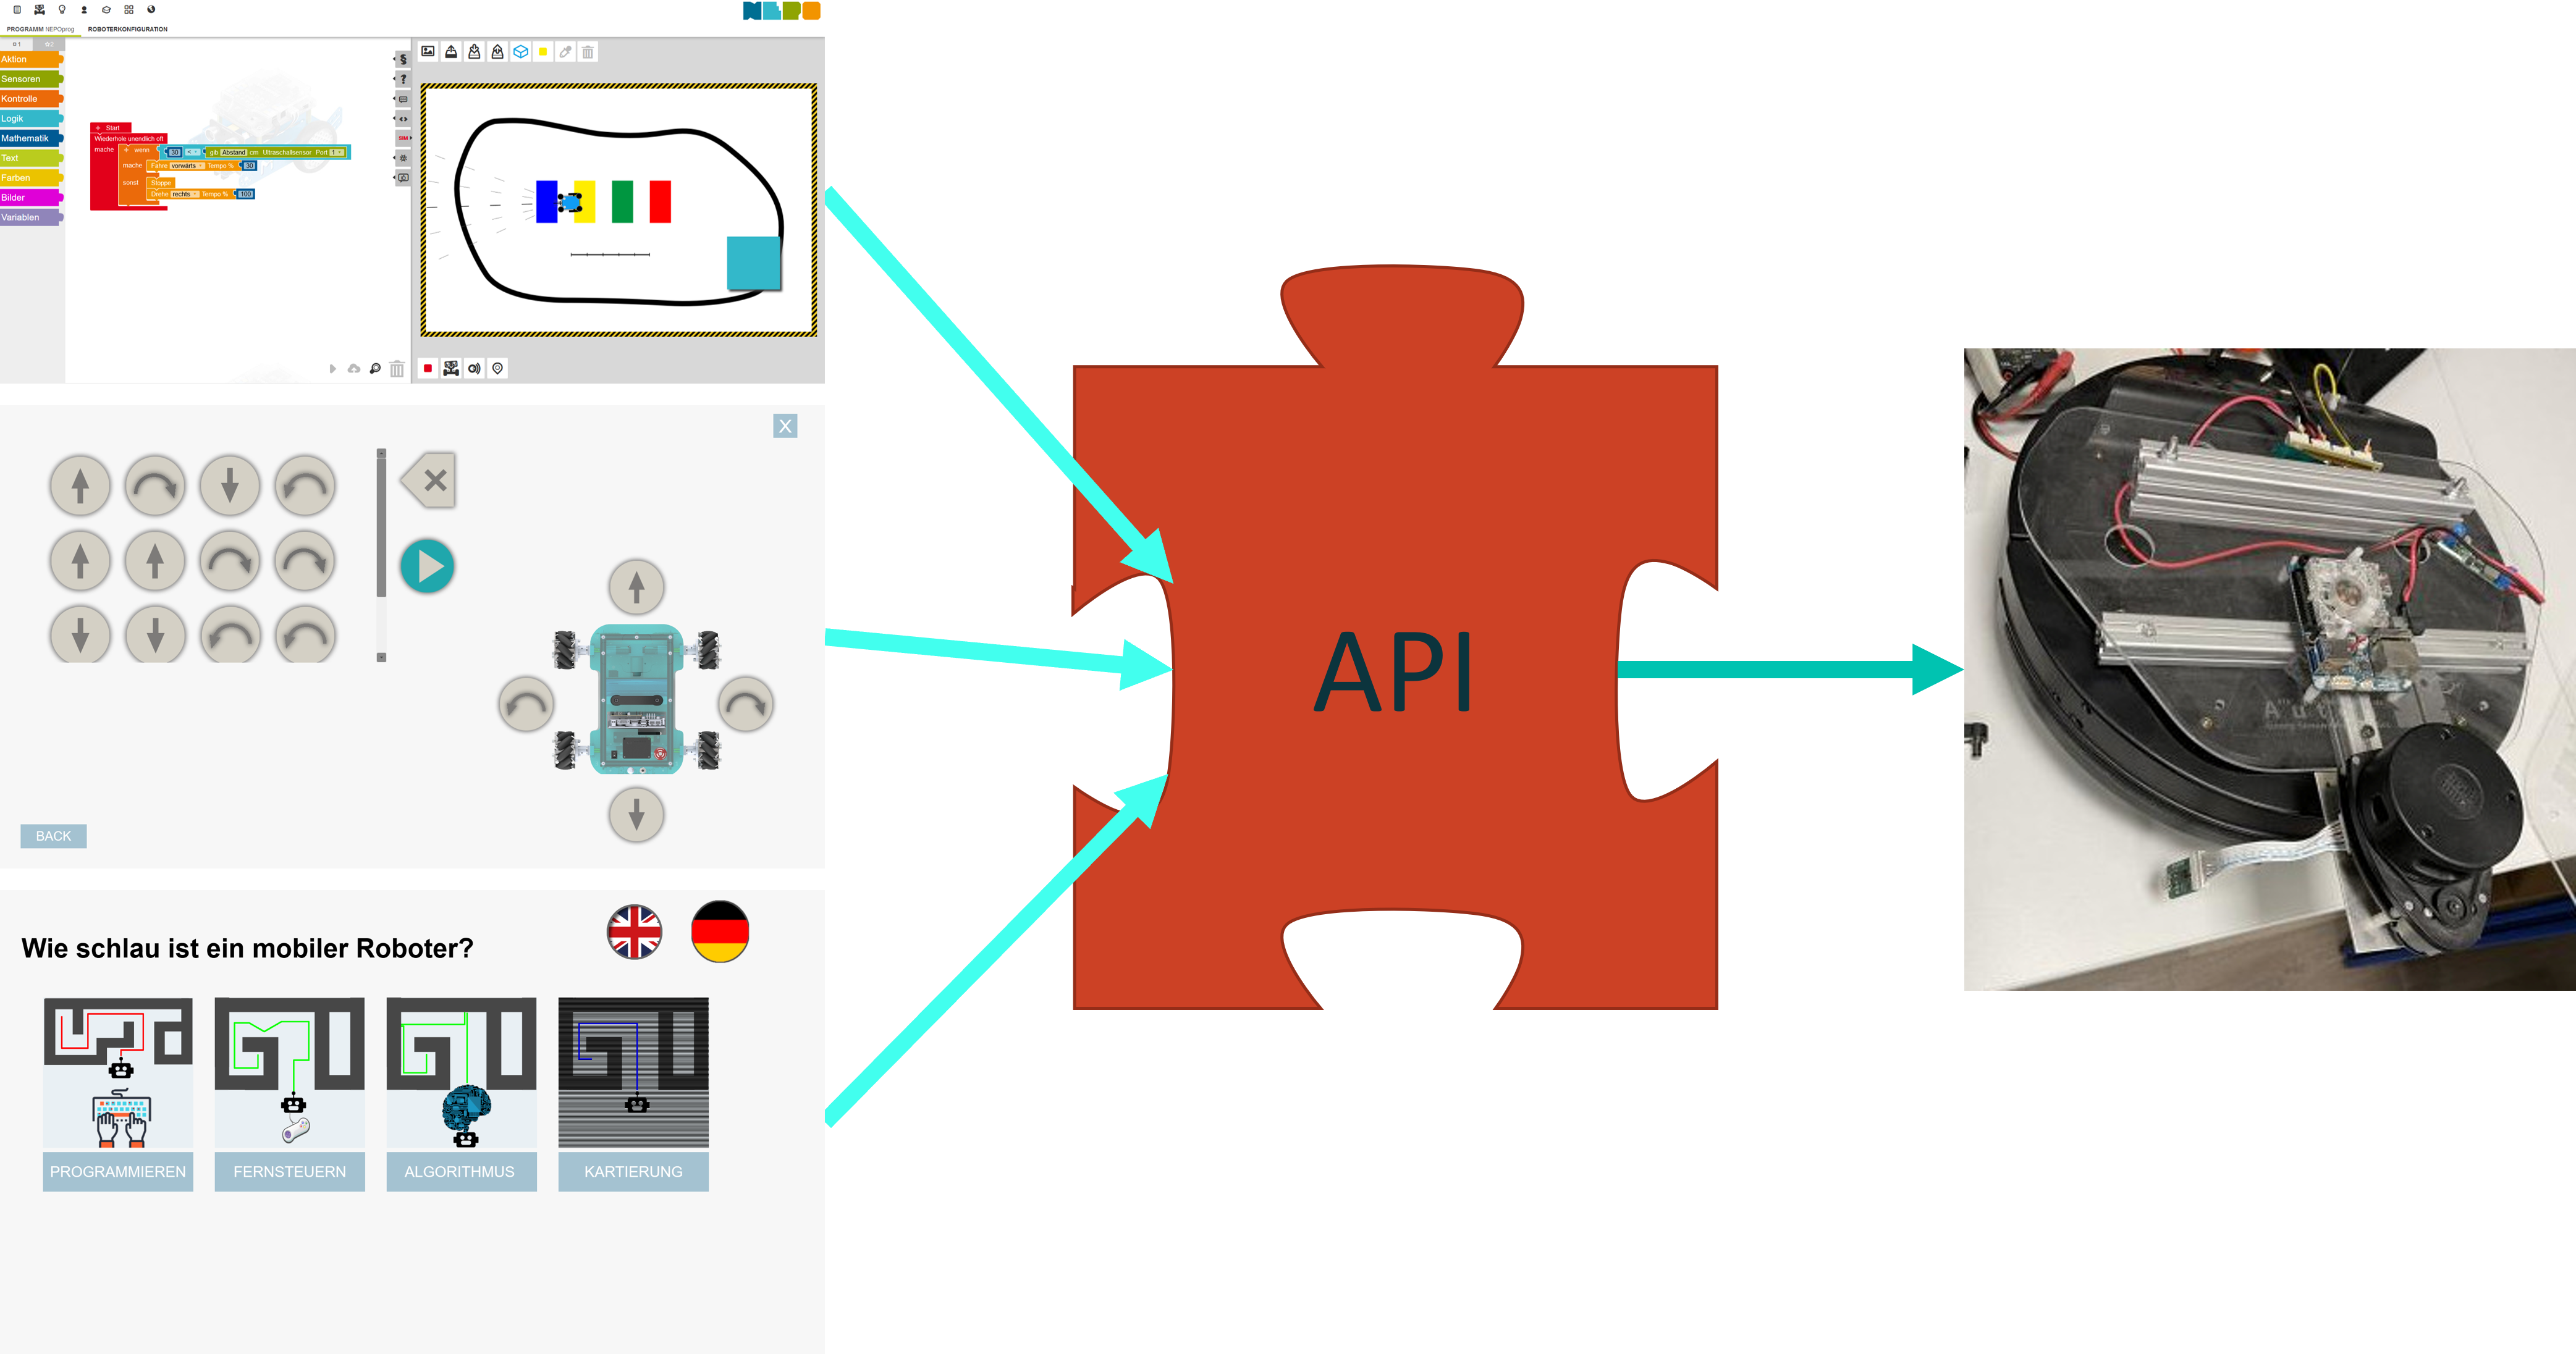
\includegraphics[width=\linewidth]{Bilder/Ergebnisse/gui_api_robot.png}
 \caption{Vereinfachte Darstellung der Kommunikation mit der API}
 \label{fig:gui_api_robot}
\end{figure}
 
Des weiteren konnte ein Ansatz für einen Algorithmus entwickelt werden der dazu dient den mobilen Roboter aus einem benutzerdefinierten Hindernisparcours zu befreien. Durch solche intelligenten Funktionalitäten können die Möglichkeiten des Machbaren an die anwendenden Personen transportiert werden. Dabei schafft diese Arbeit eine Basis und einen Grund-Wissenslevel der für weitere Funktionalitäten genutzt werden kann.
 
Die Arbeit behandelte viele kleine Punkte, die zu diesem Ergebnis führten. So konnte eine Basis geschaffen werden, die zur Weiterentwicklung herangezogen werden kann. Es können weitere Intelligenzen des mobilen Roboters implementiert werden und so spielerisch der Wissensstand der Forschung auf dem Gebiet der mobilen Roboter übermittelt werden. Die weiteren Anknüpfungspunkte dieser Arbeit könnten Kartierung mithilfe von SLAM sein. So kann durch Kartenbildung eine schnellere Navigation zur Ladestation erfolgen. Die Kartenbildung könnte sich beim Plegde-Algorithmus im Hintergrund aufbauen und im Anschluss könnte durch einen anderen Algorithmus wie \textit{A-Star} oder \textit{Dijkstra} der Pfad zurück zum Start gefunden werden.  